\newpage
\section{Alloy}
\qquad In this section, the relations, constrains and rules between elements of our data model are given. Here the alloy signatures and facts follow:\newline 
\begin{figure}[tbh]
  \begin{l}
  % Requires \usepackage{graphicx}
  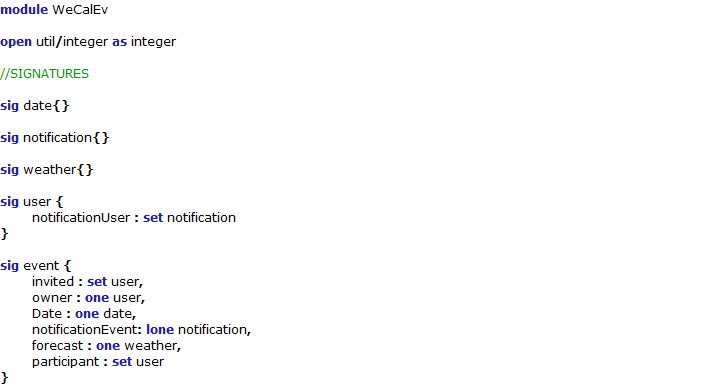
\includegraphics[width=150mm]{Code1}
  \end{l}
\end{figure}

\begin{figure}[tbh]
  \begin{l}
  % Requires \usepackage{graphicx}
  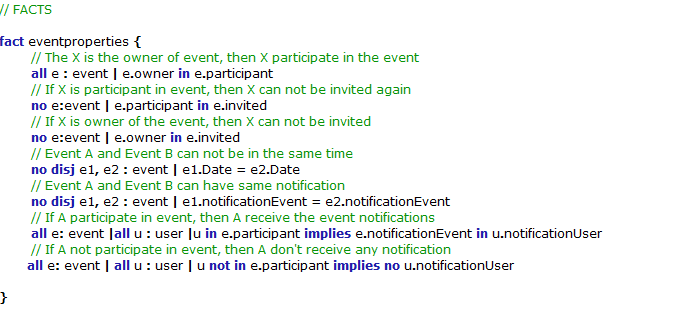
\includegraphics[width=150mm]{Code2}
  \end{l}
\end{figure}
\newpage

\begin{figure}[tbh]
  \begin{l}
  % Requires \usepackage{graphicx}
  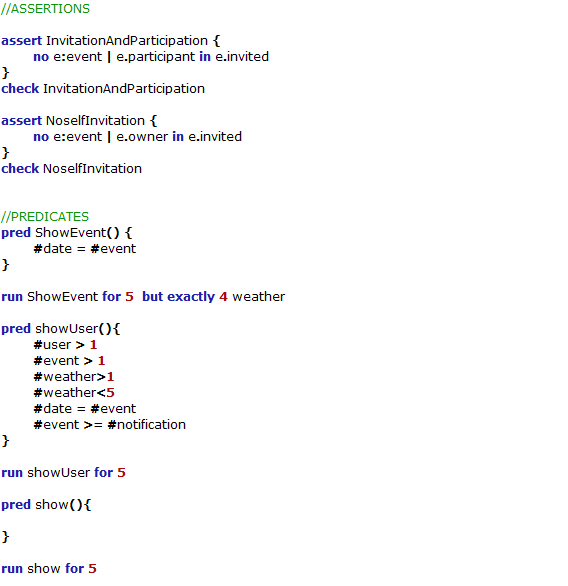
\includegraphics[width=130mm]{Code3}
  \end{l}
\end{figure}



\newpage
\qquad The execution log of the above code for every run configurations is given below:\newline
\begin{figure}[tbh]
 \begin{center}
   %Requires \usepackage{graphicx}
  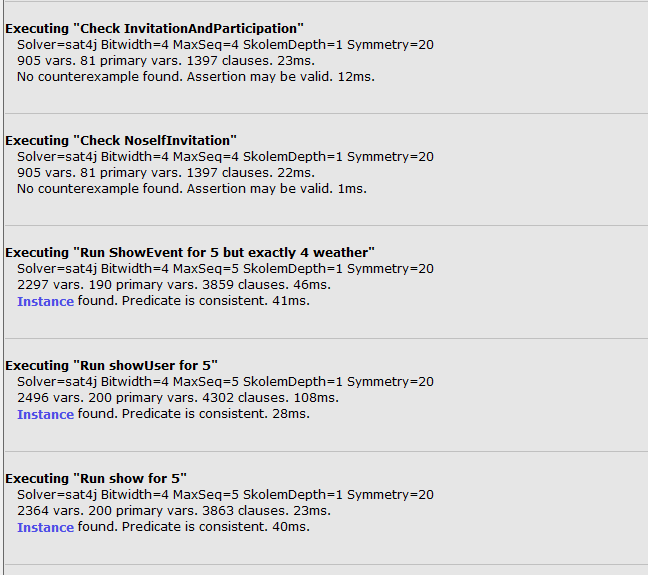
\includegraphics[width=180mm]{Alt2}
    %\caption{WeCalEvent Instance complex view}\label{Fig :}
  \end{center}
\end{figure}
\newpage
\qquad This static diagram is called metadata model. It shows all possible relations between elements without considering the facts. 
\begin{figure}[tbh]
  \begin{center}
  % Requires \usepackage{graphicx}
  \includegraphics[width=150mm]{metamodel}
    \caption{WeCalEvent metamodel}\label{Fig :}
  \end{center}
\end{figure}



\begin{figure}[tbh]
  % Requires \usepackage{graphicx}
  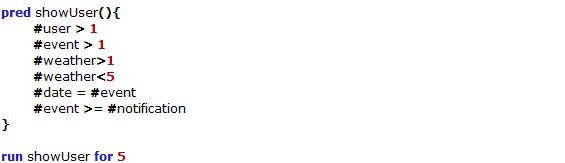
\includegraphics[width=180mm]{run}
  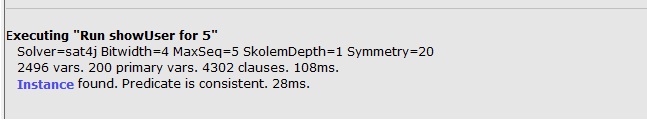
\includegraphics[width=180mm]{Alt1}

\end{figure}




\newpage

 We can see below the possible states:\\
 - If a user is invited to an event, he/she cannot be invited again and cannot be in the participant list.\\
 - The owner of an event is also a participant.\\
 - Two events can not happen on the same date.\\
 - Each event has a weather forecast.\\
 - User must be a participant of the event to receive a notification.\\



\begin{figure}[tbh]
  \begin{center}
  % Requires \usepackage{graphicx}
  \includegraphics[width=180mm]{simplified}
    \caption{WeCalEvent Instance(simplified)}\label{Fig :}
  \end{center}
\end{figure}

\newpage
This diagram provides an example of more complex relations with a couple elements more:\\


\begin{figure}[tbh]
  \begin{center}
  % Requires \usepackage{graphicx}
  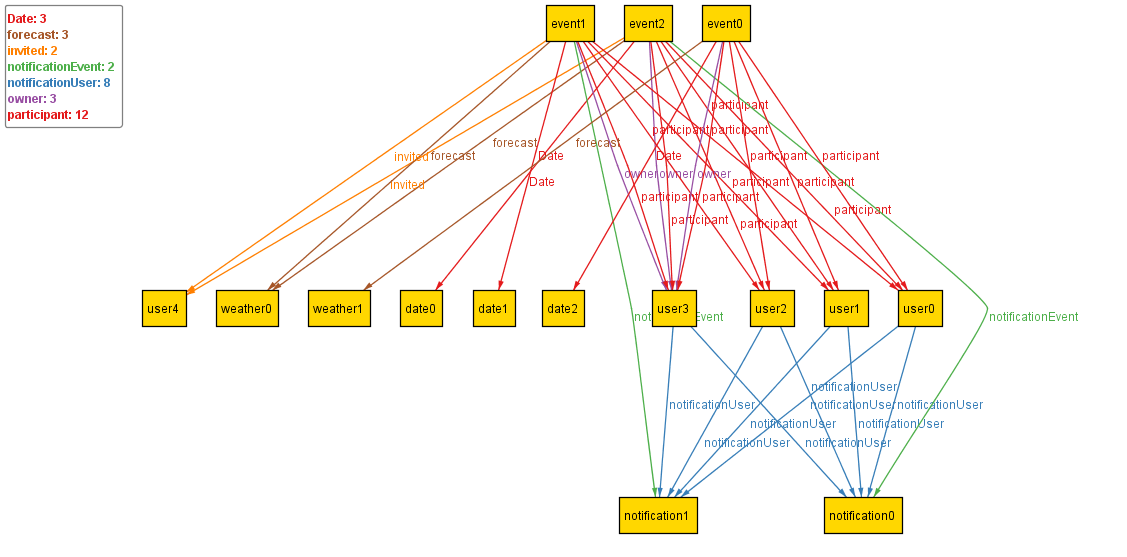
\includegraphics[width=180mm]{complex}
    \caption{WeCalEvent Instance complex view}\label{Fig :}
  \end{center}
\end{figure} 